
% Le type de votre document
\documentclass[a4paper,12pt]{report}

% Quelques packages pour le francais, vous pouvez saisir du texte accentué.
\usepackage[utf8]{inputenc} 
\usepackage[french]{babel}

% Des trucs biens pour le pdf.
\usepackage{ae}
% \usepackage{aeguill}
\usepackage{hyperref}
\usepackage{amssymb}
\usepackage{caption} 

% Pour inclure des graphiques.
\usepackage{graphicx}


% Pour faire déborder les cases d'un tableau sur plusieurs lignes.
\usepackage{multirow}
% Autres
\usepackage{amsmath}
% Des commandes perso.
%%%%%%%%%%%%%%%%%%%%%%

% J'adore l'\Crucial{Informatique} plus que tout
\newcommand{\Crucial}[1]{#1\footnote{Le concept {\bf #1} est crucial~!}}

% Faites de l'\Important{Informatique} les gars.
\newcommand{\Important}[1]{ {\em #1} }

% N'oubliez pas, \Dixit{alea jacta est}{Jules César} vaut pour tous.
\newcommand{\Dixit}[2]{\og~#1~\fg (#2)}

\newtheorem{theoreme}{Th\'{e}or\`{e}me}%[section]
\newtheorem{corollaire}{Corollaire}
\newtheorem{proposition}{Proposition}
\newtheorem{definition}{D\'efinition}%[section]
\newtheorem{remarque}{Remarque}
\newtheorem{lemmme}{Lemme}
\newtheorem{exemple}{Exemple}
\newtheorem{exercice}{Exercice}
%\newtheorem{pa}{Partie}

\begin{document}
\begin{titlepage}
\begin{center} 
    
   
\includegraphics[width=0.5\textwidth]{logo.png}\\[1cm]
   {\large Faculté des sciences Rabat}\\[0.5cm]
   {\large Licence fondamentale en Mathématiques et applications  }\\[0.5cm]
      
   % Title
   \rule{\linewidth}{0.5mm} \\[0.4cm]
   { \huge \bfseries Analyse des images par machine learning \\[0.4cm] }
   \rule{\linewidth}{0.5mm} \\[1.5cm]
      
   % Author and supervisor
   \noindent
   \begin{minipage}{0.4\textwidth}
   \begin{flushleft} \large
   \emph{Encadré par}\\
   Mr\up{} \textsc{ZIANI}\\
         
   \end{flushleft}
   \end{minipage}%
   \begin{minipage}{0.4\textwidth}
   \begin{flushright} \large
   \emph{Réalisé par :}\\
      Mr\up{} Ayoub \textsc{OUAALA}\\
   \end{flushright}
   \end{minipage}
    
\vfill
   
% Bottom of the page
{\large 2021 - 2022 }
   
\end{center}
\end{titlepage}


\section*{Remerciements}
\addcontentsline{toc}{chapter}{Remerciements}
je tiens à saisir cette occasion et adresser mes profonds remerciements et mes profondes reconnaissances à :\\

Mon encadrant Mr Ziani , pour l’orientation, la confiance, la patience qui as constitué un apport considérable sans lequel ce travail n’aurait pas pu être mené au bon port.
Son œil critique m a été très précieux pour structurer le travail et pour améliorer la qualité des différentes sections. j espère Qu’il trouve dans ce travail un hommage vivant à sa haute personnalité.\\ 

Mes vifs remerciements vont également aux membres du jury pour l’intérêt qu’ils ont porté à ma recherche en acceptant d’examiner mon travail et de l’enrichir par leurs propositions.\\ 

Mes remerciements s’étendent également à tous nos enseignants durant ces années d'études.\\
J’oublie pas mes parents pour leur contribution, leur soutien et leur patience.  mes proches et amis, qui m ont toujours encouragée au cours de la réalisation de ce projet . \\ 

Enfin, je tiens également à remercier toutes les personnes qui ont participé de près ou de loin à la réalisation de ce travail.\\ 

 
 \newpage
 
% La table des matières
\tableofcontents

% ========================================================================================================================= %
\chapter*{Introduction}
\addcontentsline{toc}{chapter}{Introduction}
% ========================================================================================================================= %

Le traitement d'images est une discipline de l'informatique et des mathématiques appliquées qui étudie les images numériques et leurs transformations, dans le but d'améliorer leur qualité ou d'en extraire de l'information.

Il s'agit d'un sous-ensemble du traitement du signal dédié aux images et aux données dérivées comme la vidéo (par opposition aux parties du traitement du signal consacrées à d'autres types de données : son et autres signaux mono dimensionnels notamment), tout en opérant dans le domaine numérique (par opposition aux techniques analogiques de traitement du signal, comme la photographie ou la télévision traditionnelles).

Dans le contexte de la vision artificielle, le traitement d'images se place après les étapes d'acquisition et de numérisation, assurant les transformations d'images et la partie de calcul permettant d'aller vers une interprétation des images traitées. Cette phase d'interprétation est d'ailleurs de plus en plus intégrée dans le traitement d'images, en faisant appel notamment à l'intelligence artificielle pour manipuler des connaissances, principalement sur les informations dont on dispose à propos de ce que représentent les images traitées (connaissance du « domaine »).

La compréhension du traitement d'images commence par la compréhension de ce qu'est une image. Le mode et les conditions d'acquisition et de numérisation des images traitées conditionnent largement les opérations qu'il faudra réaliser pour extraire de l'information. En effet, de nombreux paramètres entrent en compte.

% ========================================================================================================================= %
\chapter{\'Etat de l'art} 
% ========================================================================================================================= %

% ========================================================================================================================= %
\section{L'image numérique}
% ========================================================================================================================= %
L'image est définie comme étant une fonction $f(x,y)$ à deux dimensions, où $x$ et $y$ sont les coordonnées spatiales, et l'amplitude à tout point $(x,y)$ correspond à l'intensité ou au niveau de gris. \\
Lorsque les points $(x,y)$ et l'amplitude sont discrétisés, on parle d'image numérique ou digitale. Dans ce dernier cas la fonction $f$ est remplacée par la lettre $I$ et le couple $(x,y)$ par le couple $(i,j)$. Ainsi, une image numérique est constitué d'un ensemble de points appelés \textbf{pixels } (abréviation de \textbf{PIC}ture \textbf{El}ement). Les pixels sont approximativement rectangulaires, parfois carrés. Le pixel représente alors le plus petit élément constitutif d'une image numérique. L'ensemble de ces pixels est contenu dans un tableau à deux dimensions constituant l'image, voir la figure \ref{fig:ImageNum}.

\begin{figure}[!ht]
 	\centering
	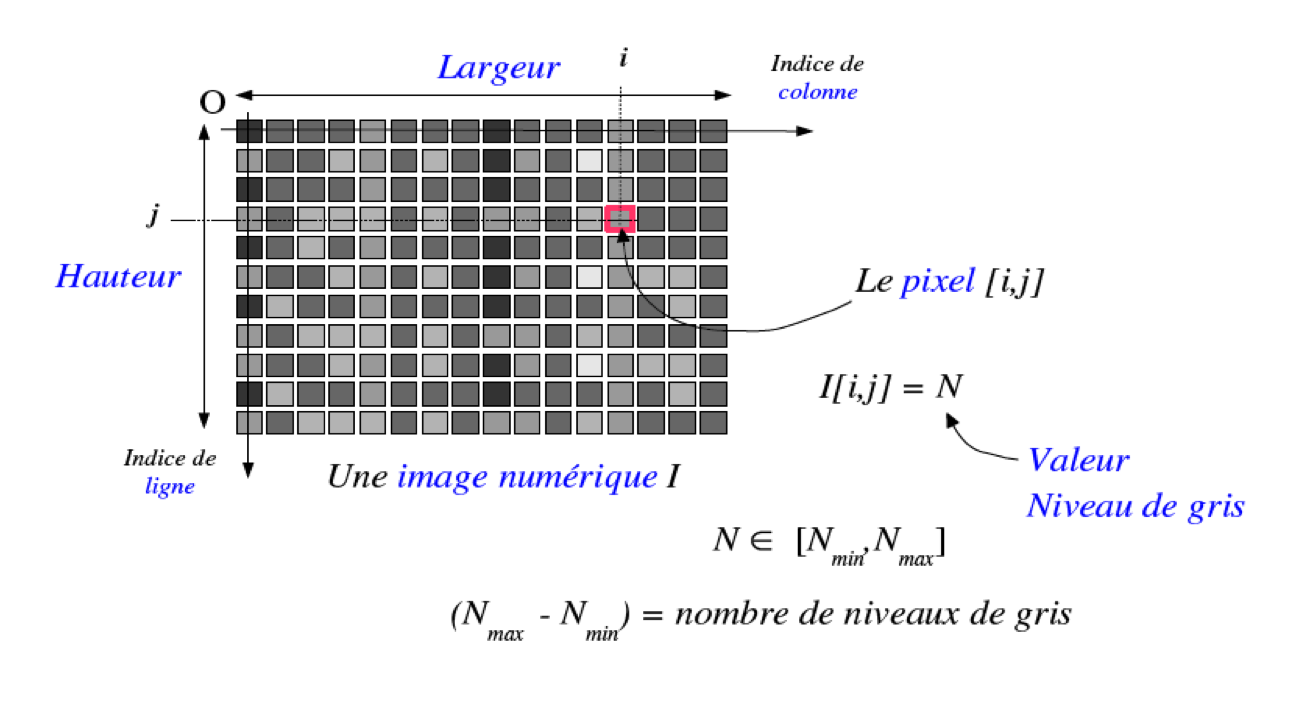
\includegraphics[scale=0.5]{ImageNum}
	\caption{Image numérique} \label{fig:ImageNum}
\end{figure}

% ========================================================================================================================= %
\subsection{Types d'images numériques}
% ========================================================================================================================= %
Selon la représentation des couleurs, nous distinguons quatre types d'images:

% ========================================================================================================================= %
\subsubsection{Images binaires}
% ========================================================================================================================= %
Pour une image binaire, chaque pixel est soit blanc soit noir, voir figure \ref{fig:ImageBinaire}. Puisqu'il y a uniquement deux valeurs pour chaque pixel, un seul bit est utilisé pour le coder.
\begin{figure}[!ht]
	\centering
	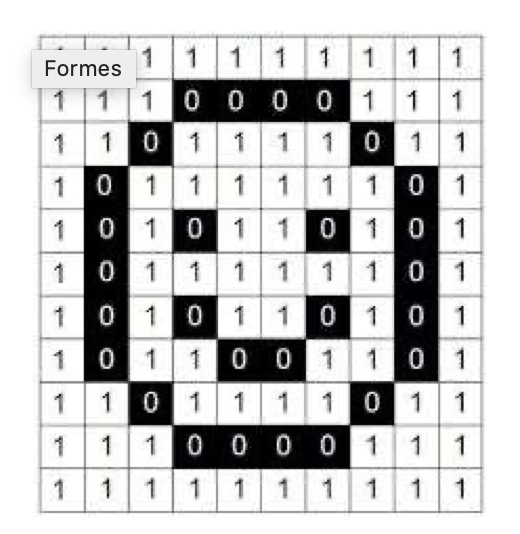
\includegraphics[scale=0.5]{ImageBinaire}
	\caption{Image binaire} \label{fig:ImageBinaire}
\end{figure}

% ========================================================================================================================= %
\subsubsection{Images en niveaux de gris}
% ========================================================================================================================= %
Pour une image en niveaux de gris, chaque pixel est un niveau de gris, allant de $0$ (noir) à $255$ (blanc). Cet intervalle de valeurs signifie que chaque pixel est codé sur $8$ bits (un octet), voir figure \ref{fig:ImageNivGris}. 
\begin{figure}[!ht]
	\centering
	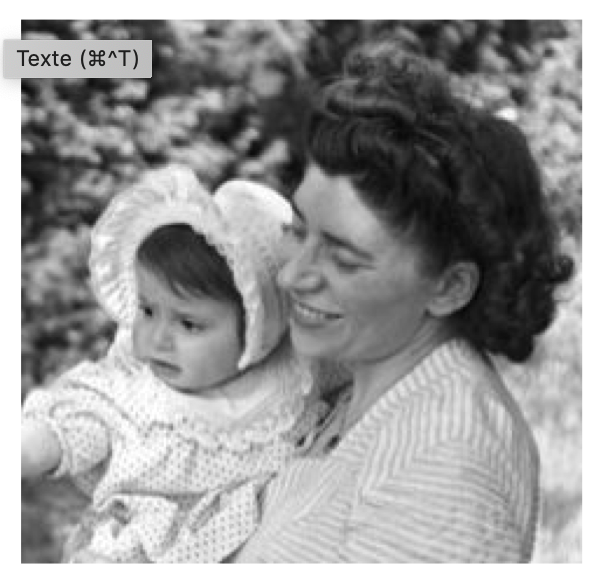
\includegraphics[scale=0.5]{ImageNivGris}
	\caption{Image en niveaux de gris} \label{fig:ImageNivGris}
\end{figure}

% ========================================================================================================================= %
\subsubsection{Images en couleurs (ou RGB)}
% ========================================================================================================================= %
Pour une image en couleurs, chaque pixel possède une couleur décrite par la quantité de rouge (R), vert (G) et bleu (B), voir figure \ref{fig:ImageCouleur}. Chacune de ces trois composantes est codée sur l'intervalle $[0,255]$, ce qui donne $255^3= 16~777~216$ couleurs possibles. Il faut donc $24$ bits pour coder un pixel. 
\begin{figure}[!ht]
	\centering
	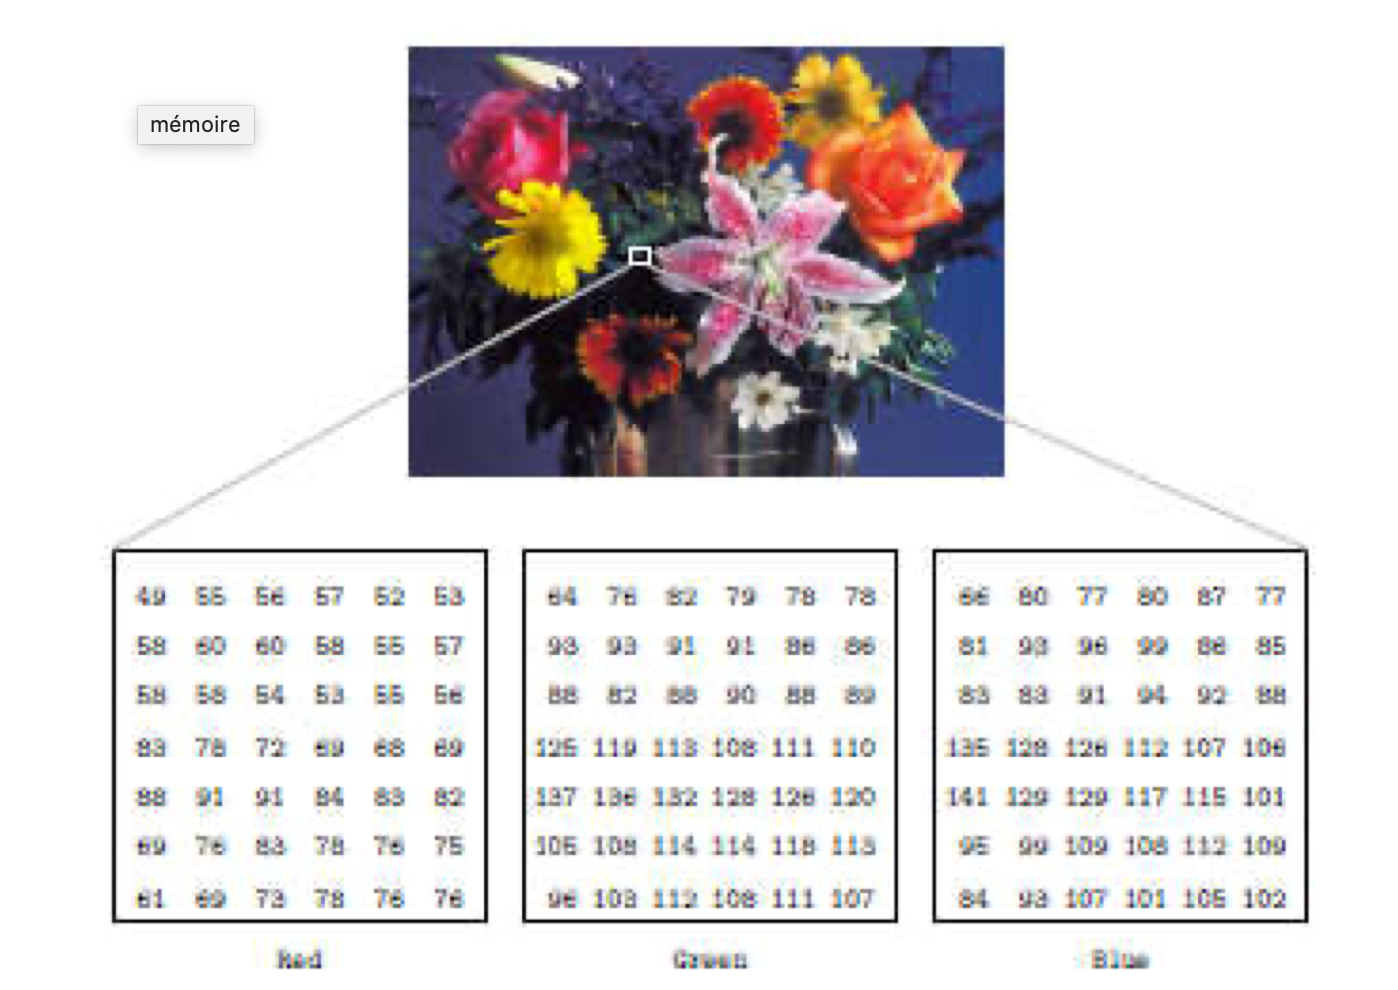
\includegraphics[scale=0.5]{ImageCouleur}
	\caption{Image en couleurs} \label{fig:ImageCouleur}
\end{figure}

% ========================================================================================================================= %
\subsection{Caractéristiques d une image}
% ========================================================================================================================= %
\subsubsection{Les pixels}
% ========================================================================================================================= %
Une image numérique est constituée d’un ensemble de points appelés pixels (abréviation de PICture Element) pour former une image.

Le pixel représente ainsi le plus petit élément constitutif d’une image numérique.

L’ensemble de ces pixels est contenu dans un tableau à deux dimensions constituant l’image :
\begin{figure}[ht]
	\centering
	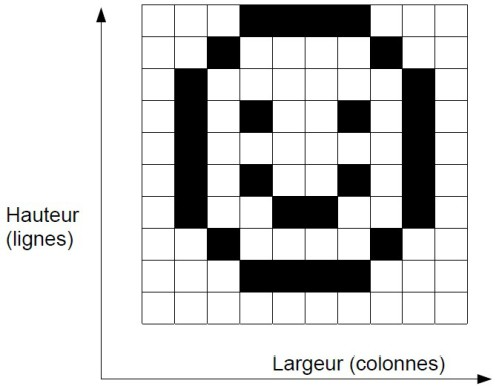
\includegraphics[width=0.5\textwidth]{matrix.jpg}
	\caption{Exemple d une image matricielle « 10 x 11 ».}
	\label{fig:matrix}
\end{figure}

% ========================================================================================================================= %
\subsubsection*{Le codage des couleurs}
% ========================================================================================================================= %
En plus de sa définition, une image numérique utilise plus ou moins de mémoire selon le codage des informations de couleur qu’elle possède.

C’est ce que l’on nomme le codage de couleurs ou profondeur des couleurs, exprimé en bit par pixel (bpp): 1, 4, 8, 16 bits…

En connaissant le nombre de pixels d’une image et la mémoire nécessaire à l’affichage d’un pixel, il est possible de définir exactement le poids que va utiliser le fichier image dans une mémoire informatique.

Formule pour calculer le poids d’une image en octet:

\begin{center}
	\textbf{Nombre de pixel total $\times$ codage couleurs (octet) = Poids (octet)}
\end{center}


Petit rappel du code binaire, utilisé par l’ordinateur pour enregistrer des informations.

« On sait que : »
\begin{itemize}
	\item 1bit = 2 possibilitées ; (0 ou 1) possibilité de coder 2 couleurs par pixel\\
	\item 2bits = 4 possibilitées ( 00 / 01 / 10 / 11 ) possibilité de coder 4 couleurs par pixel\\
	\item 4bits = 16 possibilitées ( 0000 / 0001 / 0011 / 0111 / 1111 / 0010 /0110 / 1010 /  …. ) possibilité de coder 16 couleurs par pixel\\
	\item 8bits = 256 possibilités —- codage de 256 couleurs par pixel\\
\end{itemize}

\begin{figure}[ht]
	\centering
	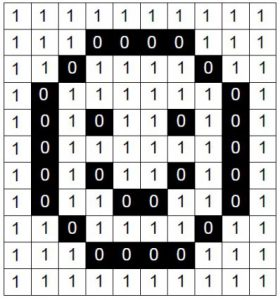
\includegraphics[width=0.5\textwidth]{zero one.jpg}
	\caption{Exemple d’image noir et blanc ou chaque pixel et codé avec un seul bit}
	\label{fig:zero.and.one}
\end{figure}

\subsection*{Histogramme d une image numérique}
\subsubsection*{Définition }
En imagerie numérique, l’histogramme représente la distribution des intensités (ou des couleurs) de l'image. C'est un outil fondamental du traitement d'images, avec de très nombreuses applications. Les histogrammes sont aussi très utilisés en photographie et pour la retouche d'images.\\

\begin{figure}[ht]
	\centering
	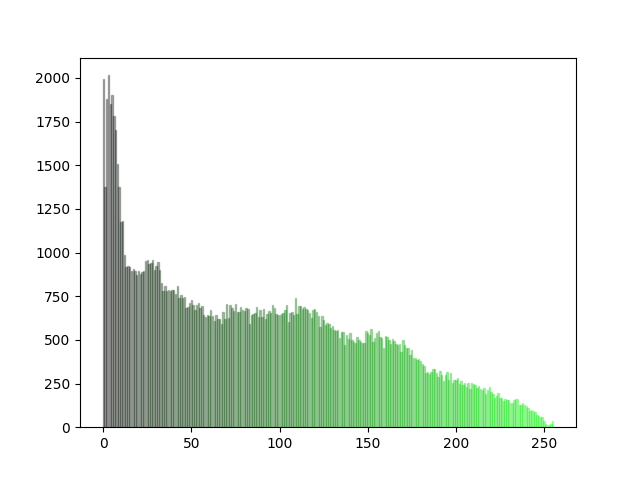
\includegraphics[width=0.8\textwidth]{Figure_1.png}
	\caption{Histogramme des degrés du vert dans une image}
	\label{fig:my_label}
\end{figure}

Les histogrammes sont en général normalisés, en divisant les valeurs de chaque classe par le nombre total de pixels de l'image \textbf{n} . La valeur d'une classe varie alors entre 0 et 1, et peut s'interpréter comme la probabilité d'occurrence de la classe dans l'image. L'histogramme peut alors être vu comme une densité de probabilité1. Pour une image {x} en niveaux de gris codée sur ${\displaystyle L}$ niveaux, on définit $n_k$ le nombre d'occurrences du niveau $x_k$. La probabilité d'occurrence d'un pixel de niveau $x_k$ dans l'image est:
\begin{center}
	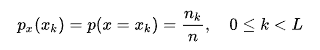
\includegraphics[width=0.7\textwidth]{probability.PNG}
\end{center}

avec \textbf{n} le nombre total de pixels de l'image, et $p_x$ définit alors l'histogramme normalisé sur [0,1].

\subsubsection*{Propriétés d'histogramme :}
Les histogrammes sont résistants à un certain nombre de transformations sur l'image. Ils sont invariants aux rotations et aux translations, ainsi que dans une moindre mesure aux changements de point de vue, et aux changements d'échelle. Les histogrammes sont en revanche sensibles aux changements d'illumination et aux conditions d'éclairage.

Pour un histogramme normalisé, la valeur de chaque classe s'interprète comme la probabilité d'occurrence de la classe dans l'image. Un histogramme normalisé somme à 1.

% ========================================================================================================================= %
\section{Machine Learning}
% ========================================================================================================================= %

Le Machine Learning ou apprentissage automatique est un domaine scientifique, et plus particulièrement une sous-catégorie de l’intelligence artificielle. Elle consiste à laisser des algorithmes découvrir des ”patterns“, à savoir des motifs récurrents, dans les ensembles de données. Ces données peuvent être des chiffres, des mots, des images, des statistiques, $\ldots$ 

Les algorithmes de Machine Learning apprennent de manière autonome à effectuer une tâche ou à réaliser des prédictions à partir de données et améliorent leurs performances au fil du temps. Une fois entraîné, l’algorithme pourra retrouver les patterns dans de nouvelles données.\\

Les algorithmes de l'apprentissage automatique se classent en deux catégories principales; on distingue entre un algorithme supervisé et un algorithme non supervisé. 


% ========================================================================================================================= %
\subsection{Apprentissage supervisé} 
% ========================================================================================================================= %
Pour l'apprentissage supervisé la machine s'apprend sur des données dont la nature des résultats est connue au préalable, c'est exactement le principe d'un enseignant supervisant le processus d'apprentissage de ses élèves ou il connait les réponses correctes et il est là pour corriger les erreurs qu'ils commettent. Cet type d'apprentissage est généralement utile dans les problèmes de \textbf{classification} et \textbf{régression}. 

% ========================================================================================================================= %
\subsubsection{Régression} 
% ========================================================================================================================= %
 En mathématiques, la régression recouvre plusieurs méthodes d’analyse statistique permettant d’approcher une variable à partir d’autres qui lui sont corrélées. Par extension, le terme est aussi utilisé pour certaines méthodes d’ajustement de courbe.
 
 En apprentissage automatique, on distingue les problèmes de régression des problèmes de classification. Ainsi, on considère que les problèmes de prédiction d'une variable quantitative sont des problèmes de régression tandis que les problèmes de prédiction d'une variable qualitative sont des problèmes de classification.
 
 La résolution de problèmes de régression est l'une des applications les plus courantes des modèles d'apprentissage automatique, en particulier dans l'apprentissage automatique supervisé. Les algorithmes sont formés pour comprendre la relation entre les variables indépendantes et un résultat ou une variable dépendante. Le modèle peut ensuite être exploité pour prédire le résultat de données d'entrée nouvelles et inédites, ou pour combler une lacune dans les données manquantes.
 
 \begin{figure}[!ht]
 	\centering
 	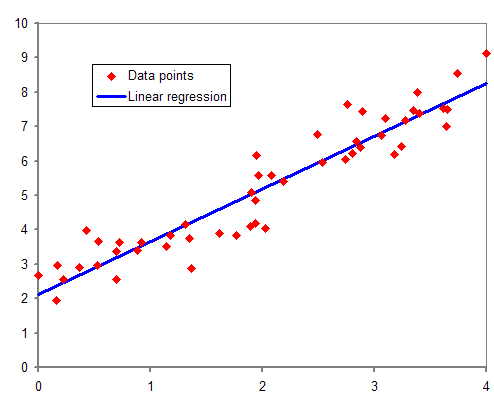
\includegraphics[width=0.6\textwidth]{regression.png}
 	\caption{Exemple de l'application de la régression}
 	\label{fig:my_label}
 \end{figure}
Parmi les types de régression, on pourra citer:
\begin{itemize}
	\item Le modèle de régression le plus connu est le modèle de \textbf{régression linéaire.}
	\item Lorsque le modèle n'est pas linéaire, on peut effectuer une régression approchée par des algorithmes itératifs, on parle de \textbf{régression non linéaire}.
	\item Si on s'intéresse au quantile conditionnel de la distribution de la variable aléatoire $y$ sachant le vecteur de variables aléatoires $y$, on utilise un modèle de \textbf{régression quantile}.
	\item Si la variable expliquée est une variable aléatoire binomiale, il est courant d'utiliser \textbf{une régression logistique ou un modèle probit.}
	\item Si la forme fonctionnelle de la régression est inconnue, on peut utiliser un modèle de \textbf{régression non paramétrique.}
\end{itemize}
 
% ========================================================================================================================= %
\subsubsection{Classification} 
% ========================================================================================================================= %
La classification est une tâche qui nécessite l'utilisation d'algorithmes d'apprentissage automatique qui apprennent à attribuer une étiquette de classe aux exemples du domaine du problème. Un exemple facile à comprendre consiste à classer les e-mails comme "spam" ou "non spam".

Il existe de nombreux types de tâches de classification que vous pouvez rencontrer dans l'apprentissage automatique et des approches spécialisées de la modélisation qui peuvent être utilisées pour chacune.



% ========================================================================================================================= %
\subsection{Apprentissage non supervisé} 
% ========================================================================================================================= %
Dans le cas de l'apprentissage non supervisé, l'algorithme apprend d'une façon totalement autonome, c'est à dire on communique des données à la machine sans lui révéler la nature des résultats, et donc c'est à l'algorithme lui même de modéliser et de représenter la structure intéressante des données. \\
On peut réduire les problèmes d'apprentissage non supervisés à deux problèmes; le problème de "\textbf{Clustering}" pour lequel on attend de la machine à faire des regroupements des données les plus homogènes possibles, et le problème de "\textbf{Association}" qui consiste à trouver des liens entre les données. 




 













% ========================================================================================================================= %
\subsection*{Clustering}
% ========================================================================================================================= %
\subsubsection{Définition }
% ========================================================================================================================= %
Le partitionnement de données (ou data clustering en anglais) est une méthode en analyse des données. Elle vise à diviser un ensemble de données en différents « paquets » homogènes, en ce sens que les données de chaque sous-ensemble partagent des caractéristiques communes, qui correspondent le plus souvent à des critères de proximité (similarité informatique) que l'on définit en introduisant des mesures et classes de distance entre objets.\\Pour obtenir un bon partitionnement, il convient d'à la fois :\\

\begin{itemize}
    \item minimiser l'inertie intra-classe pour obtenir des grappes (cluster en anglais) les plus homogènes possibles
    \item maximiser l'inertie inter-classe afin d'obtenir des sous-ensembles bien différenciés.\\
\end{itemize}

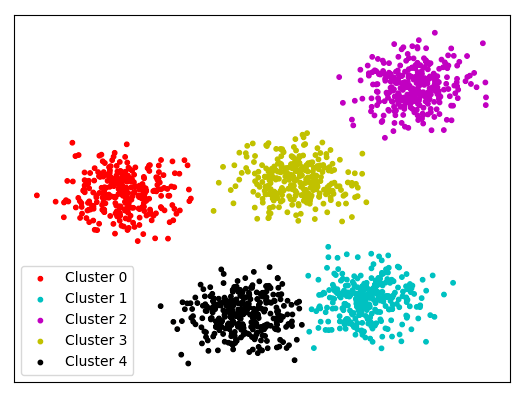
\includegraphics[width=1\textwidth]{clustering.png}



Par ailleurs, nous venons de voir les trois grandes familles de catégories du Machine Learning ( Régression, Classification, et Clustering). Désormais, vous saurez plus intuitivement de quelle catégorie il s’agit quand vous êtes confrontés à un problème d’apprentissage automatique, \\mais au long de ce projet de rechercher on s intéresse specialement a la methode du Clustering et ces applications sur l analyse des images en utilisant le language de programmation Python.











\chapter{Algorithme K-means et Analyse des images}





\section{Algorithme K-means}
\subsection{\'Etapes}
L'algorithme k-moyennes à 3 pas essentiels :


\begin{enumerate}
    \item \textbf{Initialisation: }une fois le nombre de groupes, k choisi, k barycentres sont établis dans l'espace de données, par exemple en les choisissant au hasard.
    \item \textbf{Affectation des objets aux barycentres: }chaque objet des données est affecté à son barycentre le plus proche.
    \item \textbf{Mise à jour des barycentres: }La position du barycentre de chaque groupe est mise à jour en prenant comme nouveau barycentre la position moyenne des objets appartenant audit groupe.
\end{enumerate}


répéter étape 2 et 3 jusqu'à ce que les barycentres ne bougent pas ou se déplacent en dessous d'une distance seuil à chaque étape.\\\\
Cela s'interprète mathématiquement a un problème d'optimisation et la fonction a optimiser (minimiser) est la somme des distances quadratiques de chaque objet à son barycentre du groupe qu'y appartient.

\begin{figure}[!ht]
    \centering
    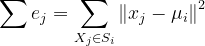
\includegraphics[width=0.3\textwidth]{CodeCogsEqn.png}
    \label{fig:equation1}
\end{figure}

Les objets sont représentés avec \textbf{d} vecteurs de dimension \textbf{n},  $x = (x_1,x_2,…,x_n)$ et le résultat de l'algorithme est \textbf{k} groupes ou la distance entre chaque vecteur et le barycentre 
du groupe qu'y appartient est minimisée l'ensemble des groupes étant \textbf{S} $= \{S_1,S_2,…,S_k\}.$
le problème peut se formuler:

\begin{figure}[h]
    \centering
    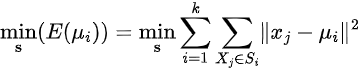
\includegraphics[width=0.5\textwidth]{equation.png}
    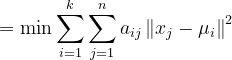
\includegraphics[width=0.4\textwidth]{suiteOfEquation.png}
    \label{fig:equation2}
\end{figure}

\begin{figure}[h]
    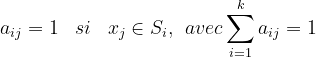
\includegraphics[width=0.5\textwidth]{CodeCogsEqn (1).png}
    \label{aij}
\end{figure}



Dans chaque mise à jour du centroïde, du point de vue mathématique, nous imposons la condition nécessaire extrême (minimale, dans ce cas) à la fonction $E(\mu_i)$ que, pour cette fonction quadratique  est :\\

\begin{figure}[h]
    \centering
    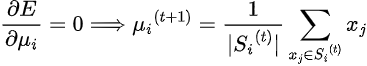
\includegraphics[width=0.5\textwidth]{second equation.png}
    \label{fig:secondEquation}
\end{figure}



et la solution consiste à prendre la moyenne de chaque élément de groupe comme nouveau centroide(barycentre). Nous avons utilisé la méthode de descente de gradient.\\

Les principaux avantages de la méthode des k-moyennes sont qu'elle est simple et rapide. Mais il est obligatoire de décider la valeur de \textbf{k} et le résultat final dépend de l'initialisation des barycentres. De plus, il ne converge pas nécessairement vers le minimum global mais vers un minimum local.


\subsection{Convergence de l'algorithme:}
Il y a un nombre fini de partitions possibles à \textbf{k} classes. De plus, chaque étape de l'algorithme fait strictement diminuer la fonction de coût, positive, et fait découvrir une meilleure partition. Cela permet d'affirmer que l'algorithme converge toujours en temps fini, c'est-à-dire termine.

Le partitionnement final n'est pas toujours optimal. De plus le temps de calcul peut être exponentiel en le nombre de points, même dans le plan. Dans la pratique, il est possible d'imposer une limite sur le nombre d’itérations ou un critère sur l'amélioration entre itérations.\\

\begin{figure}[ht]
    \centering
    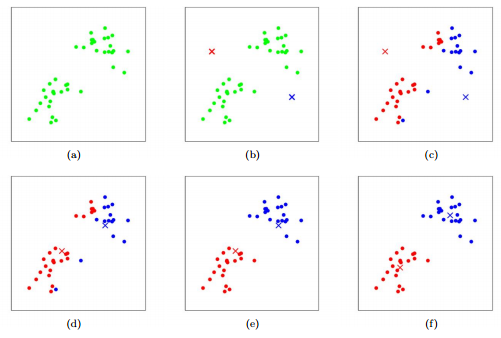
\includegraphics[width=0.7\textwidth]{convergence.png}
    \caption{exemple d'application de Kmeans sur des points de $\mathbb{R}^2$}
    \label{fig:convergence}
\end{figure}

comme on peut voir sur la figure on obtient un résultat efficace en seulement 6 opérations en appliquant kmeans a une certaines de points $(x_1,x_2,…,x_n)$ avec $x_i\in \mathbb{R}^2$ \\Mais cette efficacité dépend d'une grande degré au choix des barycentres initiales ce qui est très difficile surtout si on as pas d'informations sur les données qu'on doit travailler avec


\subsection{Avantages et inconvénients pour l'apprentissage}
Un inconvénient possible des k-moyennes pour le partitionnement est que les clusters dépendent de l'initialisation et de la distance choisie.\\

Le fait de devoir choisir a priori le paramètre k peut être perçu comme un inconvénient ou un avantage. Dans le cas du calcul des sac de mots par exemple, cela permet de fixer exactement la taille du dictionnaire désiré. Au contraire, dans certains partitionnements de données, on préférera s'affranchir d'une telle contrainte.

\subsubsection{Avantages}

\begin{itemize}
    \item -Simple
    \item -Flexible
    \item -Convient aux gros data sets
    \item -Efficace
    \item -Clusters proches
    \item -Facile à interpréter
    \item -Faible coût de calcul
\end{itemize}

\subsubsection{Inconvénients}

\begin{itemize}
    \item -Ensemble non optimal de clusters
    \item -Ordre des valeurs
    \item -Limitation des calculs
    \item -Traiter les données numériques
    \item -Problèmes de prédiction
    \item -Spécifiez les valeurs K
\end{itemize}

\subsection*{Conclusion} 
La classification K-means est une technique largement utilisée pour l’analyse par clusters de données. Cet algorithme est simple à comprendre. En outre, il fournit des résultats d’entraînement rapidement.
Cependant, ses performances ne sont généralement pas aussi compétitives que celles des autres techniques de classification sophistiquées, car de légères variations dans les données pourraient entraîner une variance des résultats élevée.\\

\section{Application de K-means pour l'analyse des images}
\subsection{Outils utilisé pour l'analyse des images}
Normalement on ne calcule pas les étapes d'un algorithme avec la main pour cela on utilise des outils scientifiques programmés en certains langages de programmation , heureusement pour le machine learning y' as plusieurs langage pour faciliter le travail en ce domaine,  on trouve parmi eux : \\
\begin{itemize}
    \item \textbf{R : }R est un langage de programmation et un logiciel libre destiné aux statistiques et à la science des données soutenu par la R Foundation for Statistical Computing\\
    \item \textbf{Matlab : } MATLAB (« matrix laboratory ») est un langage de script émulé par un environnement de développement du même nom , il est utilisé à des fins de calcul numérique. Développé par la société The MathWorks, MATLAB permet de manipuler des matrices, d'afficher des courbes et des données, de mettre en œuvre des algorithmes, de créer des interfaces utilisateurs, et peut s’interfacer avec d’autres langages comme le C, C++, Java, et Fortran.\\
    \item \textbf{Python : }Python est un langage de programmation qui peut s'utiliser dans de nombreux contextes et s'adapter à tout type d'utilisation grâce à des bibliothèques spécialisées. Il est cependant particulièrement utilisé comme langage de script pour automatiser des tâches simples mais fastidieuses,
\end{itemize}

\subsection{Installation dans l'ordinateur}
heureusement pour notre algorithme Kmeans on est issu d un package open source nommé \textbf{scikit}  (science kit) ou plusieurs outils du machine learning sont prédéfinies en plus ces outils sont faciles a interpréter dans un programme PYTHON pour résoudre les problèmes qu'on veut. \\
parmi ces outils on a la classe \textbf{KMeans} :\\

\begin{itemize}
    \item Pour installer le package \textbf{scikit} dans votre ordinateur vous devez \\insérer une des commandes suivantes.\\ 
    \begin{itemize}
        \item sur \textbf{windows} : 
            \begin{center}
                \texttt{pip install -U scikit-learn}
            \end{center}
        \item sur \textbf{linux} :
            \begin{center}
                \texttt{pip3 install -U scikit-learn}
            \end{center}
        \item sur \textbf{macOS} :
            \begin{center}
                \texttt{pip install -U scikit-learn}
            \end{center}
    \end{itemize}
    
    \item pour importer le package sur votre projet : 
    \begin{center}
        \texttt{from sklearn.* import *(Classe Voulu)}
    \end{center}
\end{itemize}

exemple pour importer spécifiquement seulement la classe \textbf{KMeans} après avoir installé le package \textbf{scikit} bien sur on insère le code suivant dans le script python qu'on travaille sur :
\begin{center}
        \texttt{from sklearn.cluster import KMeans}
\end{center}

\subsection{Utilisation de la Classe KMeans}
Voici le minimum code python pour que Kmeans nous donne des résultats :\\

\begin{figure}[ht]
    \centering
    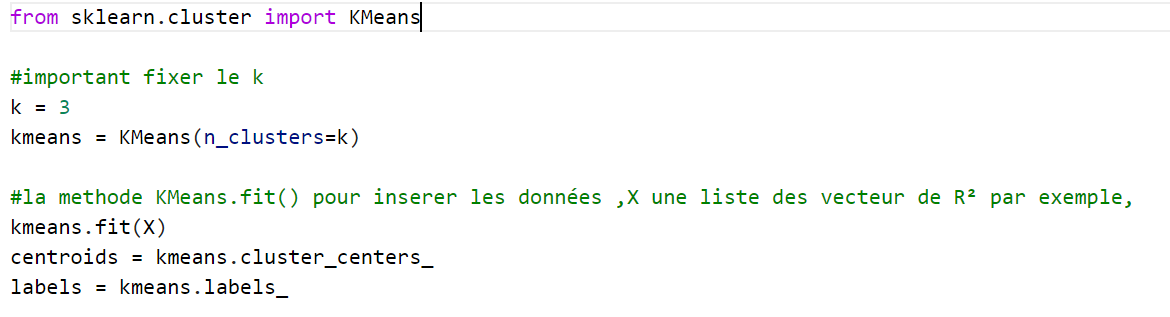
\includegraphics[width=1.2\textwidth]{etapes light.PNG}
    \caption{interprétation de KMeans sur python }
    \label{fig:kmeans etapes}
\end{figure}

\newpage
 On commence d'abord par initialiser \textbf{k} les nombre de groupes voulues(clusters), et puis on crée un objet de classe \textbf{KMeans} avec le paramètre \textbf{k} déjà initialisé, la méthode \texttt{KMeans.fit()} est où tout le calcul ce passe , et finalement on retourne les résultats sous forme de tableaux ou Listes ou seulement une seule valeur réel : \\\\
 \begin{itemize}
     \item L'attribut \texttt{cluster$\_$centers} : nous retournes les \textbf{k} barycentres résultantes de l'application de l'algorithme sur certaines données.\\
     
     \item L'attribut \texttt{labels$\_$} : nous retournes une liste qui contient le groupes résultantes de après exécution de l'algorithme mais d'une manière indirecte par exemple:
     
     si le \textbf{i}-ème vecteur appartient au \textbf{n}-ème groupe , le \textbf{i}-ème élément de \texttt{labels$\_$} aura pour valeur \textbf{n} au lieu du \textbf{i}-ème vecteur pour des raisons d'optimisation et de réduction du temps d'exécution.\\
     et ainsi de suite ...\\
     
     \item L'attribut \texttt{inertia$\_$} nous donne le pourcentage de l'erreur accumulée après la fin de l algorithme .\\
     
     \item On peut aussi spécifier le nombre d'itérations maximale qu'on veut avec le paramètre  \texttt{max$\_$iter = } dans la déclaration de l'objet du classe \textbf{KMeans}\\
     
     \item Si on veut exécuter l'algorithme plusieurs fois avant de donner le résultat il suffit de ajouter le paramètre \texttt{n$\_$init = } dans la déclaration et automatiquement le programme retournera le meilleur résultat avec le minimum d'erreur.
     
 \end{itemize} 

\subsection{La reconnaissance de l image}
L’émergence de l’intelligence artificielle fait réfléchir sur le potentiel d’évolution de nos industries et de nos métiers. De plus en plus, les entreprises ont recours à la Computer Vision (vision par ordinateur), et en particulier à la reconnaissance d’image, pour améliorer leurs processus et augmenter leur productivité. on va donc vous expliquer en quelques mots ce qu’est la reconnaissance d’image, son fonctionnement ainsi que ses différents usages.



\begin{figure}[ht]
    \centering
    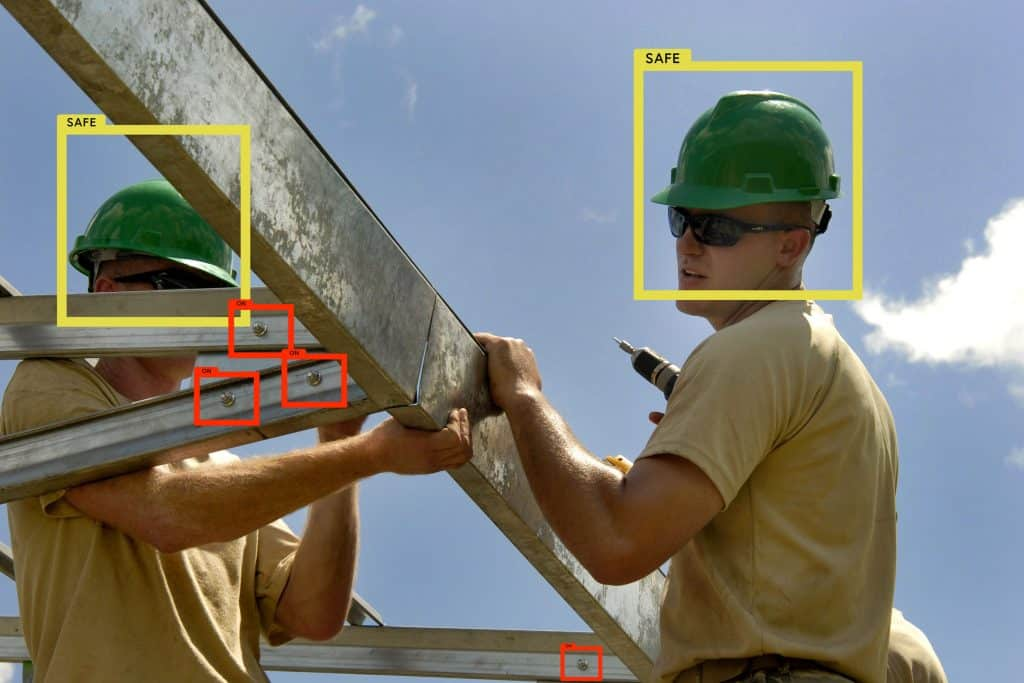
\includegraphics[width=0.6\textwidth]{image recognition.jpg}
    \caption{Exemple d'application de la reconnaissance de l image pour assurer la sécurité des ouvriers}
    \label{fig:my_label}
\end{figure}


\subsection{Définition}
La reconnaissance d’image, sous-catégorie de la Computer Vision et de l’Intelligence Artificielle, représente un ensemble de méthodes de détection et d’analyse d’images pour permettre l’automatisation d’une tâche spécifique. Il s’agit d’une technologie qui est capable d’identifier des lieux, des personnes, des objets et plusieurs autres types d’éléments au sein d’une image et d’en tirer des conclusions en les analysant.

La reconnaissance photo ou vidéo peut être réalisée à des degrés de précision différents.
Il existe donc différentes “tâches” que la reconnaissance d’image peut \\effectuer :\\

\begin{itemize}
    \item \textbf{La classification.} Il s’agit de l’identification de la “classe”, autrement dit la catégorie, à laquelle une image appartient. Une image ne peut avoir qu’une seule classe.\\
    
    \item \textbf{Le tagging.} Aussi appelé “labellisation”, il s’agit d’une tâche de classification mais à un degré de précision plus élevé. Cela va permettre de reconnaître la présence de plusieurs concepts ou objets au sein d’une image. Il est par conséquent possible d’attribuer un ou plusieurs tags à une image en particulier.\\
    
    \item \textbf{La détection.} Cela est nécessaire lorsque l’on souhaite situer un objet dans une image. Une fois la localisation réussie, un rectangle, appelée en anglais bounding box, va encadrer l’objet en question.\\
    
    \item \textbf{La segmentation.} Elle représente également une tâche de détection. La segmentation peut situer au pixel près un élément sur une image. Car dans certains cas, la précision ne peut être négligée, tel que pour le développement des voitures autonomes.\\
\end{itemize}

\chapter{Résultats numériques}

\section{Labellisation des images en utilisant K-means}
\subsection*{Définition }
La labellisation (ou classification) est l'application directe du Kmeans dans le domaine de l'analyse des images numériques, cette dernière consiste tous simplement a grouper une base de données des images an \textbf{k} groupes en précisant le \textbf{k} a priori , on peut faire cela en entrant des données sous formes de vecteur qui ont une relation directe avec les images qu'on veut classer appelées features.

\subsection*{Application et exemple }
On peut appliquer la classification sure les différents images suivantes :
\begin{figure}[ht]
    \centering
    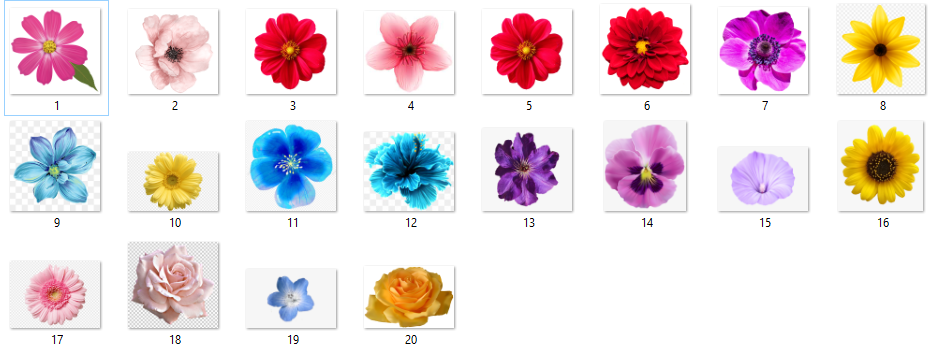
\includegraphics[width=0.9\textwidth]{dataset.PNG}
    \label{fig:dataSet}
\end{figure}

On prends en compte un vecteur de $\mathbb{R}^6$: ou les trois premiers composantes sont les moyennes des valeurs de R(rouge), G(vert), B(bleu) de chaque image, et les trois autres composantes sont les l’écart type(Standard deviation) aussi de chaque R(rouge), G(vert), B(bleu) de chaque image.\\
et voici les codes pour extraire ce vecteur sur Python :

\begin{figure}
    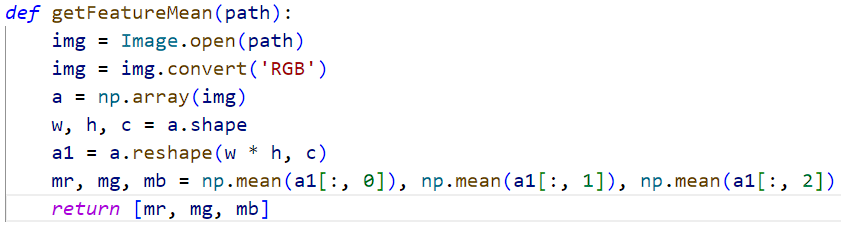
\includegraphics[width=0.7\textwidth]{mean.PNG}
    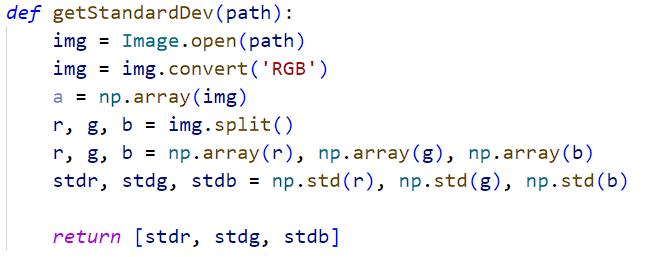
\includegraphics[width=0.7\textwidth]{stdr.PNG}
\end{figure}

On fusionne les résultats pour obtenir notre vecteur :
\begin{figure}[ht]
    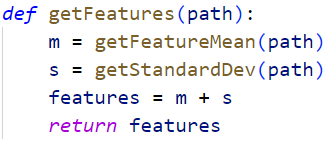
\includegraphics[width=0.4\textwidth]{fusione.PNG}
\end{figure}

Après on applique Kmeans avec le $\textbf{K} = 5$ :

\begin{figure}[ht]
    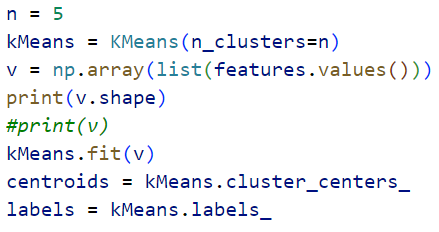
\includegraphics[width=0.6\textwidth]{kmeans.PNG}
\end{figure}

On organise les résultats et on les affiche utilisant l'interface d'affichage \texttt{matplotlib.pyplot}
en utilisant une simple boucle et la fonction \texttt{view\_clusters} que j'ai déjà défini:\newpage
\begin{figure}[ht]
    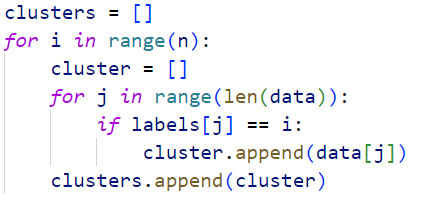
\includegraphics[width=0.5\textwidth]{results.PNG}
    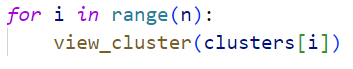
\includegraphics[width=0.5\textwidth]{showres.PNG}
\end{figure}

les résultats affichées sont : 

\begin{figure}[!h]
    
\includegraphics[width=0.7\textwidth]{1.PNG}
        \caption{Cluster 1:}
    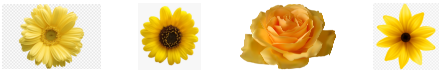
\includegraphics[width=0.6\textwidth]{2.PNG}
        \caption{Cluster 2:}
    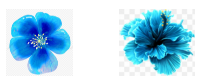
\includegraphics[width=0.3\textwidth]{3.PNG}
        \caption{Cluster 3:}
    
\includegraphics[width=0.5\textwidth]{4.PNG}
        \caption{Cluster 4:}
    
\includegraphics[width=0.6\textwidth]{5.PNG}
        \caption{Cluster 5:}
\end{figure}


\section{Quantification  d'images numériques avec k-means}
\subsection*{Définition }
La quantification est une technique de compression avec perte qui consiste à regrouper toute une groupe de valeurs en une seule. Si on quantifie la couleur d'une image, on réduit le nombre de couleurs nécessaires pour la représenter et la taille du fichier diminue.

\subsection*{Application et exemple }
D'abord on transforme l image qu'on veux quantifier en une matrice o\`u chaque composante est égale a un pixel est la valeur stockée dans ce dernier est un vecteur de $\mathbb{R}^3$ représentant les niveaux de (R, G, B) , et après en prend la matrice et on la linéarise sous forme d'un tableau qui as un longueur égale a la définition de cette image o\`u chaque élément de ce tableau est aussi un vecteur de $\mathbb{R}^3$  .   
 

\begin{figure}[ht]
    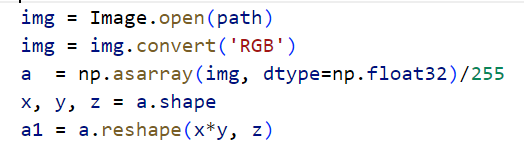
\includegraphics[width=0.6\textwidth]{pycode.PNG}
    \label{fig:open}
\end{figure}
 
 Après on applique Kmeans sur le tableau qu'on a extrait , et on change la valeur de chaque couleur par le barycentre du cluster qu'y appartient , et on reconstruit l'image résultante.

\begin{figure}[h]
    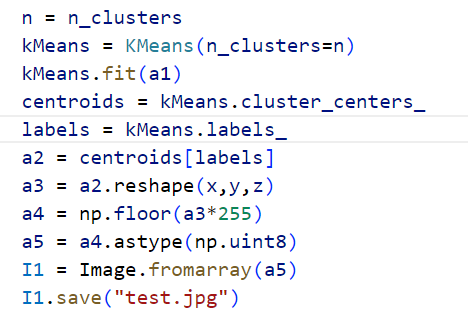
\includegraphics[width=0.5\textwidth]{pycode2.PNG}
    \label{fig:my_label}
\end{figure}

\subsection*{Exemple }
\begin{figure}[!h]
    \centering
    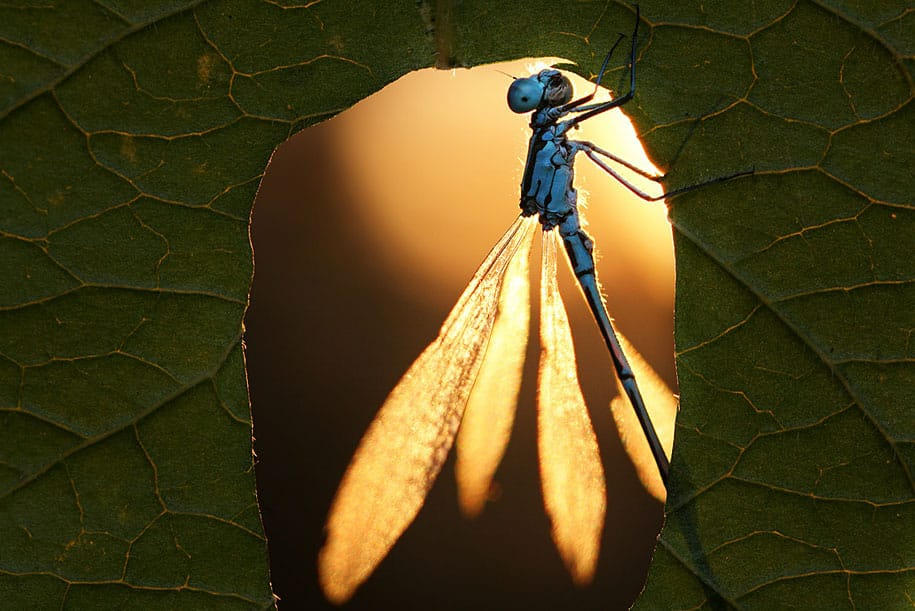
\includegraphics[width=0.4\textwidth]{insect.jpg}
    \caption{l'image avant la quantification.}
    
\includegraphics[width=0.4\textwidth]{test.jpg}
    \caption{l'image après la réduction de ces couleurs en 3.}
    \label{fig:my_label}
\end{figure}
\newpage
\section{Segmentation d'image avec kmeans }
\subsection*{Définition }
la segmentation divise une image en régions avec des propriétés internes cohérentes. Vous pouvez segmenter une image en utilisant la couleur.

Le processus est similaire à la quantification d'image. La différence est le but du regroupement de pixels : en segmentation, on regroupe les pixels pour séparer les éléments significatifs d'une image et ainsi, pouvoir extraire certaines informations quantitatives. Par exemple, calculer la taille d'une tumeur à partir d'images médicales, le pourcentage de mica dans une roche granitique, la superficie d'un lac à partir d'une photo aérienne.

\subsection*{Application et exemple }
On va utiliser la segmentation pour calculer la surface d'un lac depuis une photo aérienne.\\Pour commencer, d'abord on transforme l'image tout d'abord en la rendre en mode L c.a.d qu'elle contient que les dégrées du gris et après en réduisant ces couleurs en utilisant la quantification citée dans la dernière section.

\begin{figure}[ht]
    \centering
    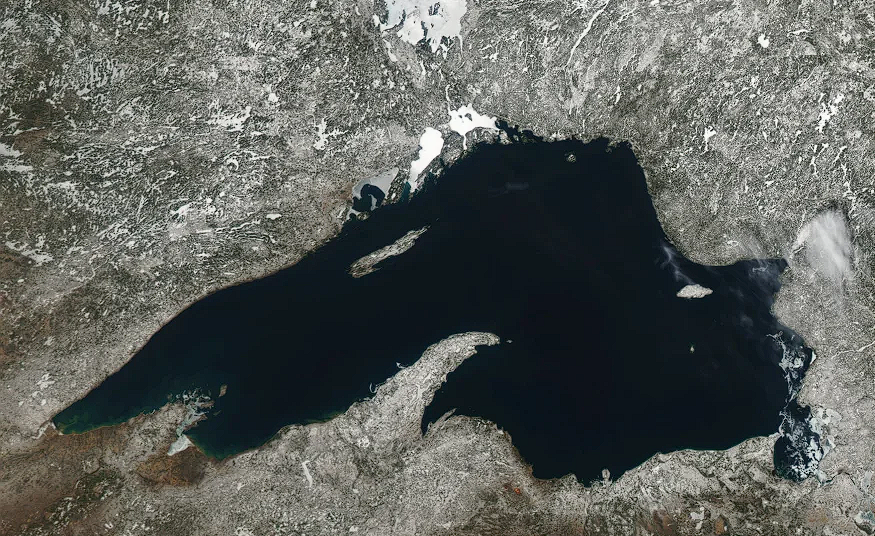
\includegraphics[width=0.6\textwidth]{lac.PNG}
    \caption{l'image du lac avant la quantification.}
    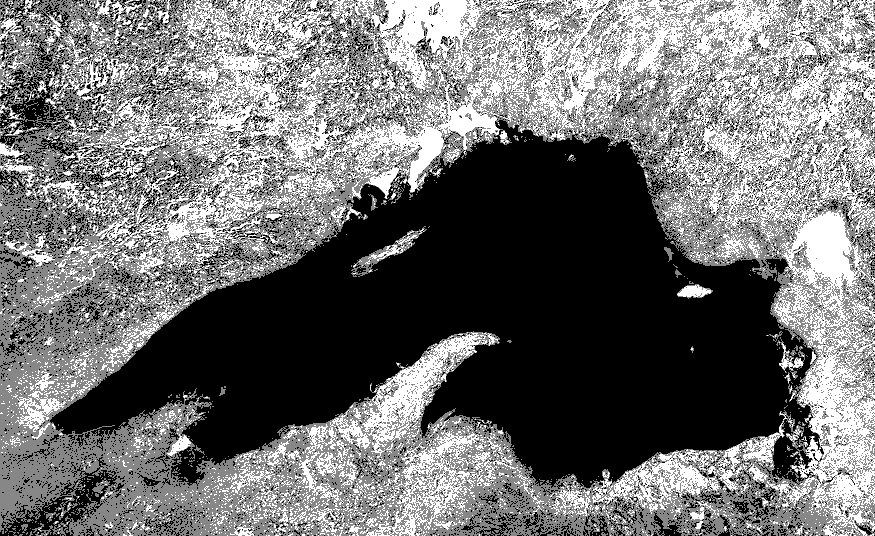
\includegraphics[width=0.6\textwidth]{lac after segmentation.PNG}
    \caption{l'image du lac après la quantification.}
\end{figure}

Comme cela on distingue le lac des autres élément, ce dernier est représenté par la surface noire.

\begin{figure}[!h]
    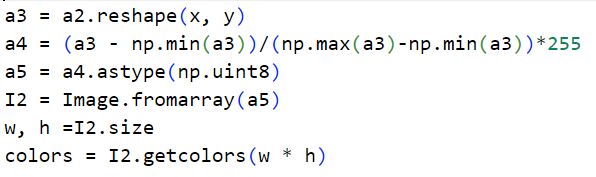
\includegraphics[width=0.7\textwidth]{recon.PNG}
\end{figure}

\begin{figure}[!h]
    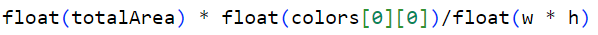
\includegraphics[width=0.8\textwidth]{area.PNG}
\end{figure}

ou \texttt{totalArea} représente la surface totale en $Km$ et \texttt{colors[0][0]} est combien de pixels occupe le noir en la divisant par \texttt{w * h} on obtient \\le pourcentage du noir par rapport a l'image totale.

les résultat finale est obtenu en $Km$ , est représente la surface du lac .
% Bibliographie
\begin{thebibliography}{99}
	\bibitem{ref1}https://fr.wikipedia.org/wiki/Apprentissage\_non\_supervisé
    \bibitem{ref2}https://mrmint.fr/machine-learning-applications
    \bibitem{ref3}https://fr.wikipedia.org/wiki/Traitement\_d'images
    \bibitem{ref4}https://fr.wikipedia.org/wiki/Histogramme\_(imagerie\_numérique)
    \bibitem{ref5}https://www.lossendiere.com/2016/08/31/caracteristiques-dune-image-numerique/
    \bibitem{ref6}https://fr.wikipedia.org/wiki/K-moyennes
    \bibitem{ref7}https://analyticsinsights.io/k-means/
    \bibitem{ref8}https://www.unioviedo.es/compnum/labs/new/kmeans.html\#:\~:text=K-means\%20is\%20an\%20unsupervised,the\%20group\%20or\%20cluster\%20centroid
    \bibitem{ref9}https://deepomatic.com/fr/quest-ce-que-la-reconnaissance-dimage
    \bibitem{ref10}https://fr.wikipedia.org/wiki/Histogramme\_(imagerie\_numérique)\\
    
    lien pour le code python et la base de données :\\
    \bibitem{ref11}https://github.com/ouaala-ayoub/PFE
    
\end{thebibliography}

% La fin du document 

\end{document}
